\chapter{System Analysis}

\section{Requirement Analysis}
The following requirements define what SEDS must do and the quality constraints it must satisfy.

\textbf{Functional Requirements:}
\begin{itemize}
  \item \textbf{User Authentication:} Secure login and signup with JWT and role-based access (Admin, Responder, Citizen); guest auto-provisioning for unauthenticated SOS submissions.
  \item \textbf{Station Management:} Admin can create, view, and manage emergency stations with PostGIS point locations.
  \item \textbf{Zone Management:} Admin can draw service zone polygons on the map or upload a GeoJSON file.
  \item \textbf{Responder Management:} Admin can create, view, edit, and delete responder accounts with station assignment.
  \item \textbf{Map View:} Landing page displays all station locations and zone boundaries on an interactive MapLibre GL map; responder dashboard shows radar visualization (pulsing rings) of pending incidents.
  \item \textbf{SOS Request:} Citizen submits emergency request by category; system auto-assigns the responsible station via zone containment or nearest-distance fallback.
  \item \textbf{Atomic Incident Claiming:} Responder claims an incident atomically; concurrent claims are rejected via Postgres row-level locking to prevent double-assignment.
  \item \textbf{Incident Lifecycle:} Incidents progress through four states (Pending, Responding, Arrived, Resolved) with responder action buttons to transition between states.
  \item \textbf{Real-Time Status Notification:} Status changes are pushed to citizens and responders in real time via Server-Sent Events over Redis pub/sub, with 5-second polling fallback for resilience.
\end{itemize}

\textbf{Non-Functional Requirements:}
\begin{itemize}
  \item \textbf{Performance:} Spatial triage (ST\_Contains) completes in under 500ms; claim operation completes in under 100ms even under concurrent load.
  \item \textbf{Security:} JWT in HTTP-only cookies; bcrypt password hashing; RBAC on all protected endpoints; row-level locking prevents unauthorized concurrent claims.
  \item \textbf{Availability:} Docker health checks ensure automatic container restart; polling fallback maintains eventual consistency if SSE disconnects.
  \item \textbf{Portability:} Entire stack deploys with a single Docker Compose command; no external service dependencies (all containerized).
  \item \textbf{Real-Time Latency:} Status notifications delivered within 1 second for connected SSE clients, within 5 seconds via polling.
\end{itemize}

\section{Feasibility Analysis}
\begin{itemize}
  \item \textbf{Technical Feasibility:} Node.js, PostGIS, MapLibre GL, Redis, and Server-Sent Events are mature open-source tools well-suited to the system's requirements; row-level locking is native to PostgreSQL and battle-tested in production systems.
  \item \textbf{Economic Feasibility:} All software dependencies are open-source with no licensing cost; deployment requires a single low-cost VPS or on-premises server.
  \item \textbf{Operational Feasibility:} The citizen SOS flow requires no more than two interactions; the admin polygon tool is map-driven and intuitive; responder dashboard is push-based (minimal polling overhead).
  \item \textbf{Schedule Feasibility:} A 6-sprint Agile timeline has been completed with 2-week sprint cycles; all core objectives delivered.
\end{itemize}

\section{Analysis Diagrams}
SEDS is developed using the Agile methodology with six two-week sprints.

\subsection{Gantt Chart}
\begin{figure}[h]
  \centering
  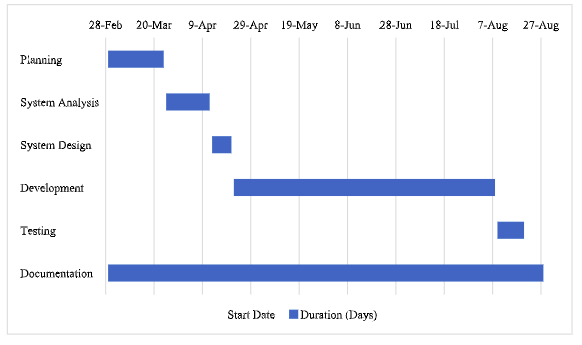
\includegraphics[width=\textwidth]{Graphics/gannt-chart.png}
  \caption{Gantt Chart of Project Timeline}
  \label{fig:gantt}
\end{figure}
\FloatBarrier

\subsection{ER Diagram}
\begin{figure}[h!]
  \centering
  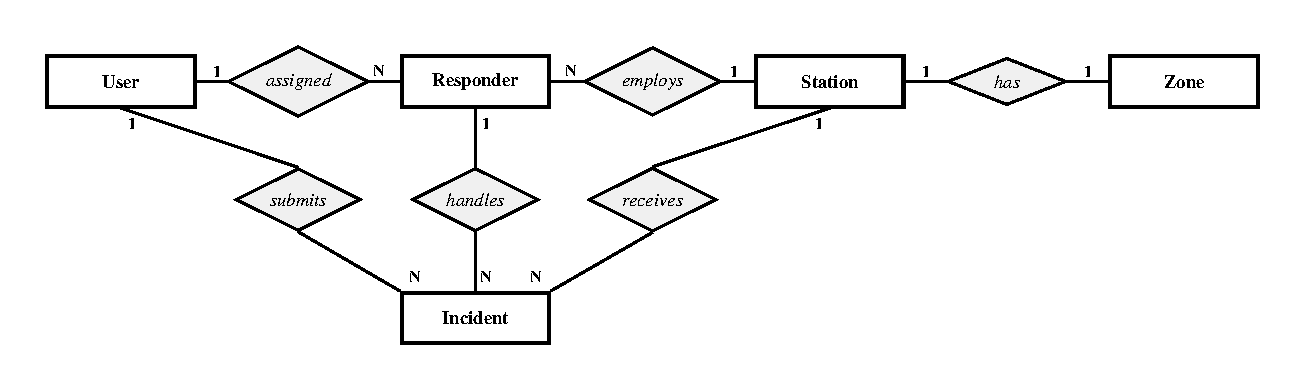
\includegraphics[width=0.9\textwidth]{Graphics/ER.pdf}
  \caption{Logical ER Diagram: User, Responder, Station, Zone, and Incident entities with relationships}
  \label{fig:er}
\end{figure}
\FloatBarrier

\begin{figure}[h]
  \centering
  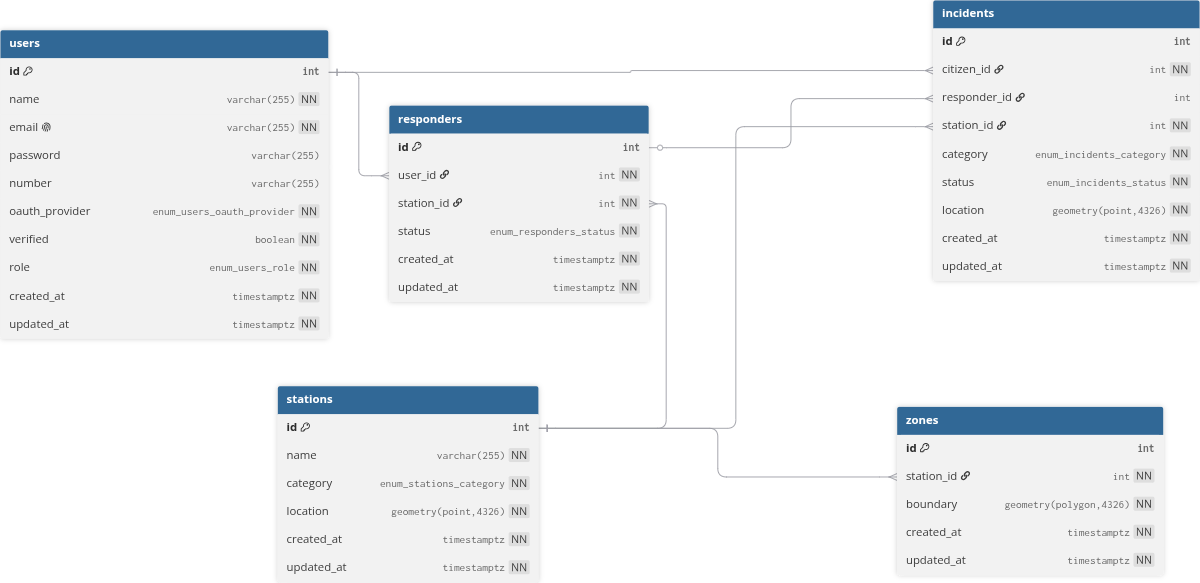
\includegraphics[width=\textwidth]{Graphics/phy_er.png}
  \caption{Physical ER Diagram}
  \label{fig:phyer}
\end{figure}
\FloatBarrier

\subsection{DFD Level 0}
\begin{figure}[h!]
  \centering
  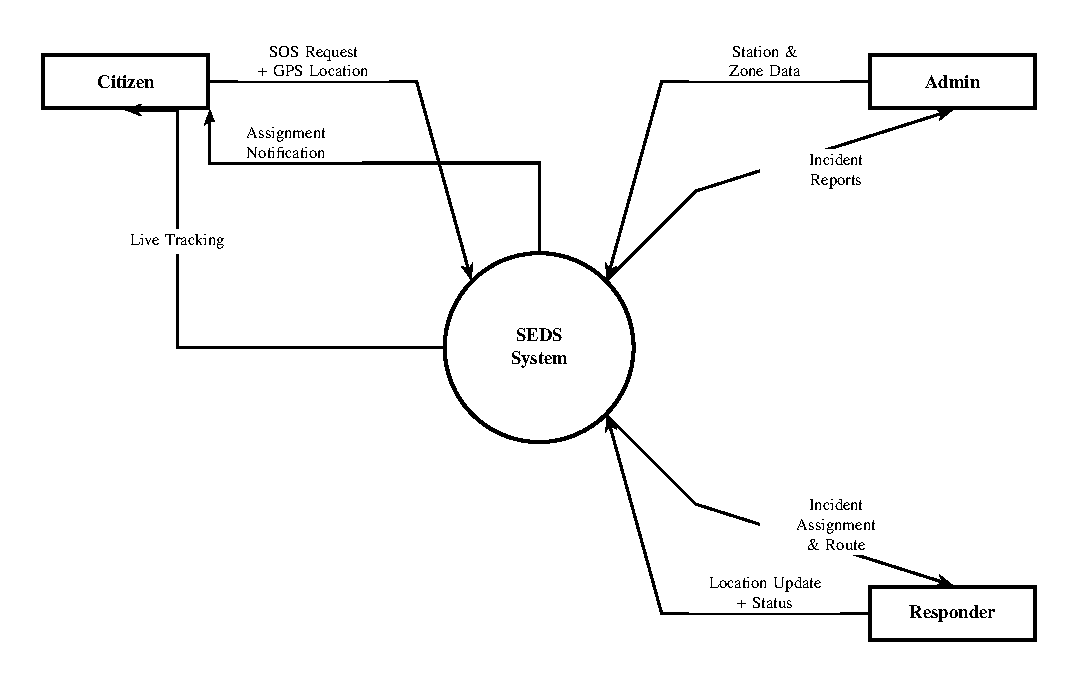
\includegraphics[height=0.4\textheight]{Graphics/level0.pdf}
  \caption{DFD Level 0: System boundary showing citizen, admin, responder interactions with SEDS}
  \label{fig:dfd0}
\end{figure}
\FloatBarrier

\newpage

\subsection{DFD Level 1}
\begin{figure}[h!]
  \centering
  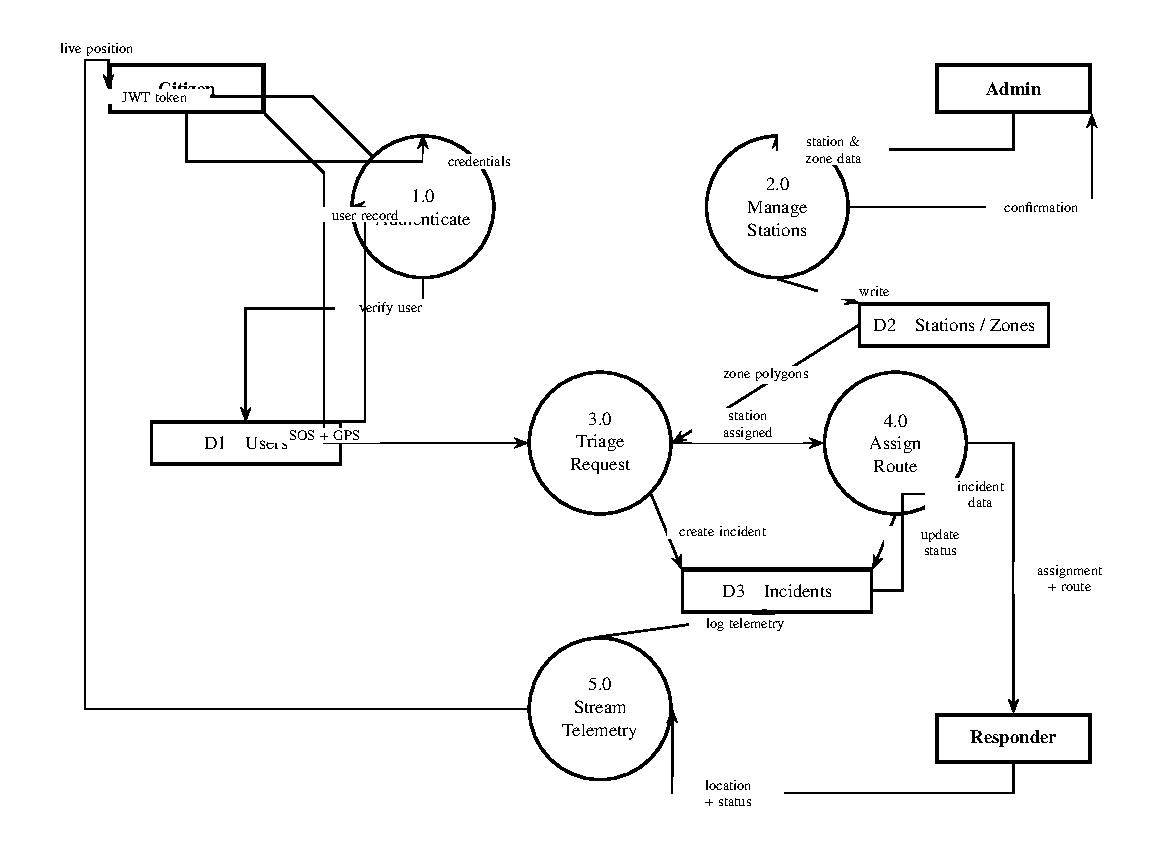
\includegraphics[height=0.4\textheight]{Graphics/level1.pdf}
  \caption{DFD Level 1: Five key processes - Authentication, Station Management, Triage, Claim \& Dispatch, and Status Push Notifications}
  \label{fig:dfd1}
\end{figure}
\FloatBarrier
